%%%%%%%%%%%%%%%%%%%%%%%%%%%%%%%%%%%%%%%%%
% Beamer Presentation
% LaTeX Template
% Version 1.0 (10/11/12)
%
% This template has been downloaded from:
% http://www.LaTeXTemplates.com
%
% License:
% CC BY-NC-SA 3.0 (http://creativecommons.org/licenses/by-nc-sa/3.0/)
%
%%%%%%%%%%%%%%%%%%%%%%%%%%%%%%%%%%%%%%%%%

%----------------------------------------------------------------------------------------
%	PACKAGES AND THEMES
%----------------------------------------------------------------------------------------

\documentclass{beamer}

\mode<presentation> {

% The Beamer class comes with a number of default slide themes
% which change the colors and layouts of slides. Below this is a list
% of all the themes, uncomment each in turn to see what they look like.

\usetheme{default}
%\usetheme{AnnArbor}
%\usetheme{Antibes}
%\usetheme{Bergen}
%\usetheme{Berkeley}
%\usetheme{Berlin}
%\usetheme{Boadilla}
%\usetheme{CambridgeUS}
%\usetheme{Copenhagen}
%\usetheme{Darmstadt}
%\usetheme{Dresden}
%\usetheme{Frankfurt}
%\usetheme{Goettingen}
%\usetheme{Hannover}
%\usetheme{Ilmenau}
%\usetheme{JuanLesPins}
%\usetheme{Luebeck}
%\usetheme{Madrid}
%\usetheme{Malmoe}
%\usetheme{Marburg}
%\usetheme{Montpellier}
%\usetheme{PaloAlto}
%\usetheme{Pittsburgh}
%\usetheme{Rochester}
%\usetheme{Singapore}
%\usetheme{Szeged}
%\usetheme{Warsaw}

% As well as themes, the Beamer class has a number of color themes
% for any slide theme. Uncomment each of these, in turn, to see how it
% changes the colors of your current slide theme.

%\usecolortheme{albatross}
%\usecolortheme{beaver}
%\usecolortheme{beetle}
%\usecolortheme{crane}
%\usecolortheme{dolphin}
%\usecolortheme{dove}
%\usecolortheme{fly}
%\usecolortheme{lily}
%\usecolortheme{orchid}
%\usecolortheme{rose}
%\usecolortheme{seagull}
%\usecolortheme{seahorse}
%\usecolortheme{whale}
%\usecolortheme{wolverine}
%\usecolortheme{structure}

%\setbeamertemplate{footline} % To remove the footer line in all slides uncomment this line
%\setbeamertemplate{footline}[page number] % To replace the footer line in all slides with a simple slide count uncomment this line

%\setbeamertemplate{navigation symbols}{} % To remove the navigation symbols from the bottom of all slides, uncomment this line
}
\usepackage{fontspec}
\usepackage{bibentry}
\usepackage{graphicx} % Allows including images
\usepackage{booktabs} % Allows the use of \toprule, \midrule and \bottomrule in tables

\setmainfont{ArialMT}
%\setbeamertemplate{frametitle}[default][center]

% 加导航条
\useoutertheme[width=3\baselineskip,right]{sidebar}
% 目录标数字
\setbeamertemplate{section in toc}[sections numbered] 
% 无序列表用实心点
\setbeamertemplate{itemize item}{\(\bullet \)}
% 设置每页标题格式
% \setbeamertemplate{frametitle}
%   {\vspace{-0.5cm}
%    \insertframetitle
%    \vspace{-0.5cm}}
% 去掉下面没用的导航条
%\setbeamertemplate{navigation symbols}{}
% 设置页脚格式
% \makeatother
% \setbeamertemplate{footline}
% {
%   \leavevmode%
%   \hbox{%
%   \begin{beamercolorbox}[wd=.4\paperwidth,ht=2.25ex,dp=1ex,center]{author in head/foot}%
%     \usebeamerfont{author in head/foot}\insertshortauthor
%   \end{beamercolorbox}

%   \begin{beamercolorbox}[wd=.6\paperwidth,ht=2.25ex,dp=1ex,center]{title in head/foot}%
%     \usebeamerfont{title in head/foot}\insertshorttitle\hspace*{13em}
%     \insertframenumber{} / \inserttotalframenumber\hspace*{0ex}
%   \end{beamercolorbox}}

%   \vskip0pt%
% }
% \makeatletter

% 定义颜色
\definecolor{alizarin}{rgb}{0.82, 0.1, 0.26} % 红色
%\definecolor{DarkFern}{HTML}{407428} % 绿色
%\colorlet{main}{DarkFern!100!white} % 第一种设置方法
\colorlet{main}{red!70!black} % 第二种设置方法
\definecolor{bistre}{rgb}{0.24, 0.17, 0.12} % 黑色
\definecolor{mygrey}{rgb}{0.52, 0.52, 0.51} % 灰色
%\colorlet{main}{green!50!black}
\colorlet{text}{bistre!100!white}

% 不同元素指定不同颜色,fg是本身颜色,bg是背景颜色,!num!改变数值提供渐变色
\setbeamercolor{title}{fg=main}
\setbeamercolor{frametitle}{fg=main}
\setbeamercolor{section in toc}{fg=text}
\setbeamercolor{normal text}{fg=text}
\setbeamercolor{block title}{fg=main,bg=mygrey!14!white}
%\setbeamercolor{block body}{fg=black,bg=mygrey!10!white}
\setbeamercolor{block body}{fg=text}
\setbeamercolor{qed symbol}{fg=main} % 证明结束后的框颜色
\setbeamercolor{math text}{fg=black}
% 设置页脚对应位置颜色
\setbeamercolor{author in head/foot}{fg=black, bg=mygrey!5!white}
\setbeamercolor{title in head/foot}{fg=black, bg=mygrey!5!white}
\setbeamercolor{structure}{fg=main, bg=mygrey!10!white} % 设置sidebar颜色

% 左右页间距的排版
% \def\swidth{2.3cm}
% \setbeamersize{sidebar width right=\swidth}
% \setbeamersize{sidebar width left=\swidth}
% \setbeamerfont{title in sidebar}{size=\scriptsize}
% \setbeamerfont{section in sidebar}{size=\tiny}

%----------------------------------------------------------------------------------------
%	TITLE PAGE
%----------------------------------------------------------------------------------------

\title[Exercise Recommendation]{Research on High School Math Exercise Recommendation Based on Graph Neural Network} % The short title appears at the bottom of every slide; the full title is only on the title page

\author{Wangzhihui Mei} % Your name
\institute[UOW] 
{
University of Wollongong \\ % Your institution for the title page
\medskip
\textit{maywzh@gmail.com} % Your email address
}
\date{\today} % Date, can be changed to a custom date

\begin{document}

\begin{frame}
  \titlepage % Print the title page as the first slide
\end{frame}

\begin{frame}
  \frametitle{Overview} % Table of contents slide, comment this block out to remove it
  \tableofcontents % Throughout your presentation, if you choose to use \section{} and \subsection{} commands, these will automatically be printed on this slide as an overview of your presentation
\end{frame}

%----------------------------------------------------------------------------------------
%	PRESENTATION SLIDES
%----------------------------------------------------------------------------------------

%------------------------------------------------
\section{Introduction}
%------------------------------------------------
\subsection{Research Background}
\begin{frame}
  \frametitle{Background}
  \begin{itemize}
    \item Knowledge State Monitoring
    \item Learning Resource Recommendation
    \item High School Math
  \end{itemize}
\end{frame}

%------------------------------------------------
\subsection{Existing Problems}
\begin{frame}
  \frametitle{Problems}
  \begin{description}
    \item[Disorganized exercise] Exercises lacking knowledge tags
    \item[Knowledge evaluation] Description of second item
    \item[Exercise recommendation] Description of third item
  \end{description}
  %\framesubtitle{}
  % \begin{itemize}
  %   \item Corpus
  %   \item Hard to evaluate the knowledge mastery status
  %   \item Difficult to find appropriate exercise for improving knowledge mastery
  % \end{itemize}
\end{frame}
%------------------------------------------------
\subsection{Research Cores}
\begin{frame}
  \frametitle{Research Cores}
  \begin{block}{Exercise knowledge labelling}
    A multi-knowledge point labelling algorithm for high school mathematics exercises based on bidirectional LSTM and graph neural network.
  \end{block}
  \begin{block}{Knowledge tracing}
    A knowledge tracing model based on Transformer architecture with graph attention network embedding.
  \end{block}
  \begin{block}{Exercise recommendation}
    A mathematical exercise recommendation model based on Matching-Ranking algorithm.
  \end{block}
\end{frame}
%------------------------------------------------
\section{Proposed Model}
\subsection{Exercise Knowledge Labelling}
\begin{frame}
  \frametitle{Exercise Knowledge Labelling}
  \framesubtitle{Architecture}
  \begin{figure}
    \caption{Model architecture}
    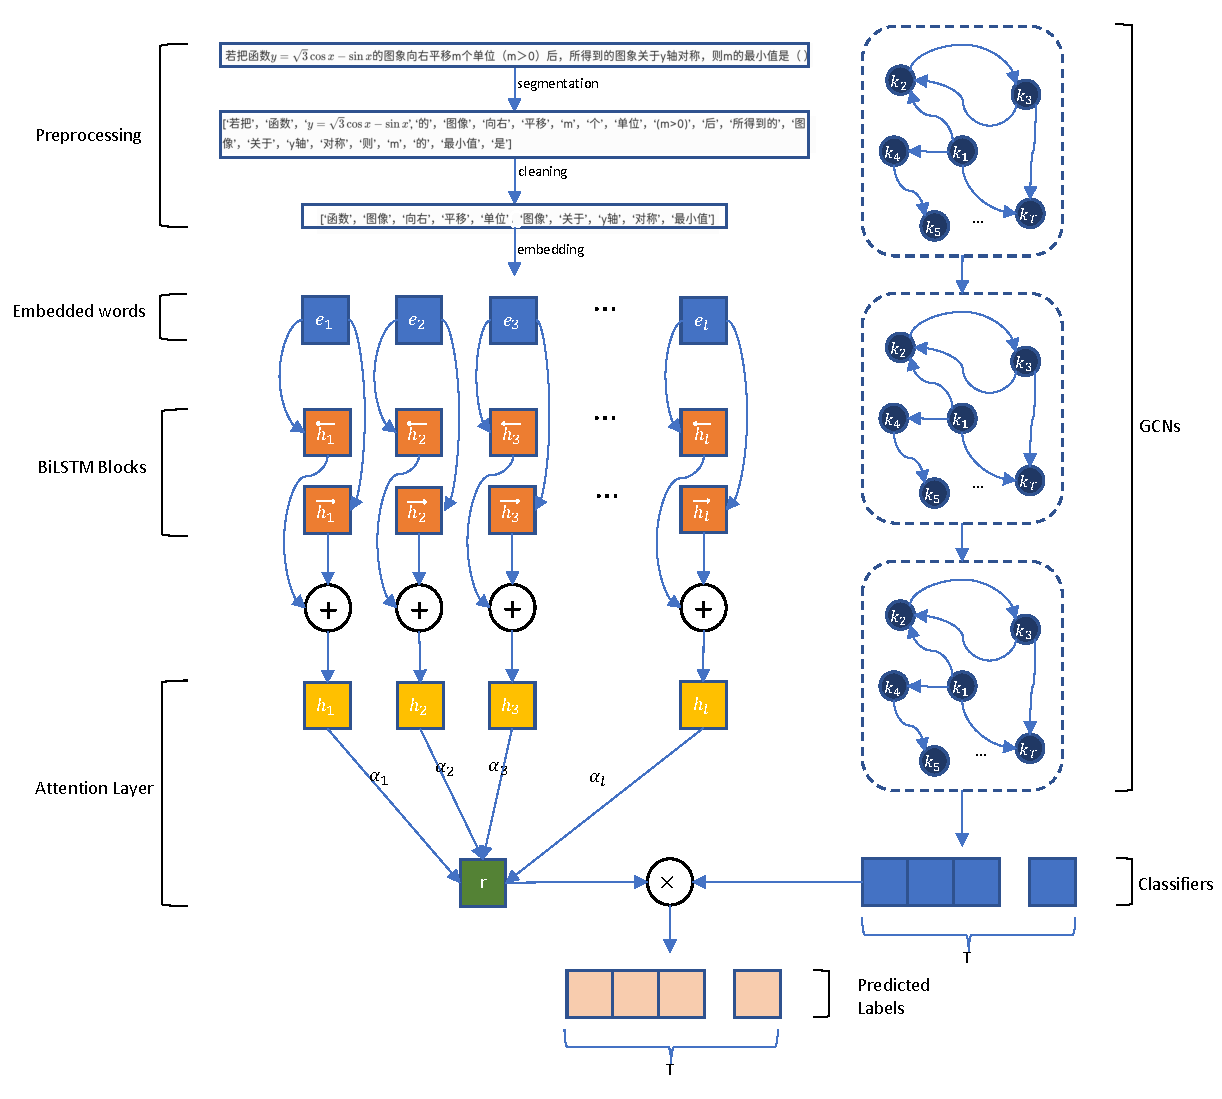
\includegraphics[width=0.9\textwidth]{figures/ch2-model-architecture.pdf}
  \end{figure}

\end{frame}
%------------------------------------------------

\begin{frame}
  \frametitle{Exercise Knowledge Labelling}
  \begin{columns}[c] % The "c" option specifies centered vertical alignment while the "t" option is used for top vertical alignment
    \column{.45\textwidth} % Left column and width
    \textbf{Heading}
    \begin{enumerate}
      \item Statement
      \item Explanation
      \item Example Table~\ref{tbl:t1}
    \end{enumerate}
    \column{.5\textwidth} % Right column and width
  \end{columns}



\end{frame}


\begin{frame}
  \frametitle{Knowledge Tracing}

\end{frame}

%------------------------------------------------

\begin{frame}
  \frametitle{Exercise Recommendation}
  \begin{block}{Block 1}
    content
  \end{block}
  \begin{block}{Block 2}
    content
  \end{block}
  \begin{block}{Block 3}
    content
  \end{block}
\end{frame}



%------------------------------------------------
\begin{frame}
  \frametitle{Table}
  \begin{table}
    \caption{Table caption}\label{tbl:t1}
    \begin{tabular}{l l l}
      \toprule
      \textbf{Treatments} & \textbf{Response 1} & \textbf{Response 2} \\
      \midrule
      Treatment 1         & 0.0003262           & 0.562               \\
      Treatment 2         & 0.0015681           & 0.910               \\
      Treatment 3         & 0.0009271           & 0.296               \\
      \bottomrule
    \end{tabular}
  \end{table}
\end{frame}

%------------------------------------------------

\begin{frame}
  \frametitle{Theorem}
  \begin{theorem}[Mass-energy equivalence]
    \(E = mc^2\)
  \end{theorem}
\end{frame}

%------------------------------------------------

% \begin{frame}[fragile] % Need to use the fragile option when verbatim is used in the slide
%   \frametitle{Verbatim}
%   \begin{example}[Theorem Slide Code]
%     \begin{verbatim}
% \begin{frame}
% \frametitle{Theorem}
% \begin{theorem}[Mass--energy equivalence]
% $E = mc^2$
% \end{theorem}
% \end{frame}\end{verbatim}
%   \end{example}
% \end{frame}

%------------------------------------------------
\section{Result}
\begin{frame}
  \frametitle{Figure}
  Uncomment the code on this slide to include your own image from the same directory as the template .TeX file.
  %\begin{figure}
  %\includegraphics[width=0.8\linewidth]{test}
  %\end{figure}
\end{frame}

%------------------------------------------------

\begin{frame}% Need to use the fragile option when verbatim is used in the slide
  \frametitle{Citation}
  This statement requires citation~\cite{shamir2010learning}.
\end{frame}

%------------------------------------------------

% \begin{frame}
%     \frametitle{References}
%     \footnotesize{
%         \begin{thebibliography}{99} % Beamer does not support BibTeX so references must be inserted manually as below
%             \bibitem[Smith, 2012]{p1} John Smith (2012)
%             \newblock Title of the publication
%             \newblock \emph{Journal Name} 12(3), 45 -- 678.
%         \end{thebibliography}
%     }
% \end{frame}

\begin{frame}[allowframebreaks]{References}
  %\bibliographystyle{plain}
  \bibliographystyle{amsalpha}
  %\bibliography{mybeamer} also works
  \bibliography{./ref.bib}
\end{frame}

%------------------------------------------------

\begin{frame}
  \Huge{\centerline{The End}}
\end{frame}

%----------------------------------------------------------------------------------------

\end{document}